\documentclass[bibliography=totocnumbered]{article}
\usepackage{lmodern}
\usepackage{amssymb,amsmath}
\usepackage{ifxetex,ifluatex}
\usepackage{fixltx2e}
\usepackage[utf8]{inputenc}
\usepackage{t1enc}
\usepackage[magyar]{babel}
\usepackage{hyperref}

\usepackage{graphicx,grffile}

\usepackage{parskip}
\usepackage[table]{xcolor}
\usepackage{pgf,tikz,pgfplots}
\pgfplotsset{compat=1.15}
\usepackage{mathrsfs}
\usetikzlibrary{arrows}


\makeindex

\begin{document}


\begin{titlepage} 
	\center {\Huge \bf Szakdolgozat} \vfill {\huge Congame} \\[20pt] {\Large Bordák Tamás} \vfill  \vfill {\Large 2015} 
\end{titlepage}

\tableofcontents
\newpage
\section{Bevezetés}

A számítógép mára az életünk része lett, ezért mindenkinek ismernie kell
a személyi számítógép különböző részeit és azok funkcióit. Napjainkra
minden korosztály fogékonnyá és nyitottá vált a számítógép használatára.
Az alapvető digitális intelligencia nélkülözhetetlen eszközzé nőtte ki
magát a munkában, az információ áramlásban és a szórakozásban is.

A szórakozás fogalma generációról generációra változik. Modern
világunkban számítógépek segítik nemcsak a munkát, hanem a
kikapcsolódást is. A mozgalmas hétköznapok közepette el is felejtjük,
hogy milyen lehetőségek vannak karnyújtásnyira. Így számítógépeink
szórakoztató képességeit hajlamosak vagyunk figyelmen kívül hagyni.

A fejlődő technika újabb és újabb vívmányai lehetővé teszik az egyre
látványosabb grafikai szoftverek hétköznapi használatát. Ennek a
legnagyobb piaca a játékipar.

A számítógépes játékok egy része lélegzetelállító grafikai elemeket
tartalmaz, míg más játékok éppen a képi egyszerűségük, közérthetőségük
miatt sikeresek.

A játéklehetőségek széles spektrumának kínálatában ki-ki megtalálja az
igényeinek legmegfelelőbb számítógépes játékokat, melyek napjainkban
népszerű időtöltésnek bizonyulnak.


\subsection{ Mitől jó egy játék}

Nem a grafika határozza meg egy játék élvezeti értékét, ezt napjaink
egyik legnépszerűbb játéka a Minecraft is igazolja. Alapvető grafikai
elemeket használhatunk ötleteink megépítésére, akár barátainkkal vagy
más játékosokkal közreműködve.

Minden idők legsikeresebb játékaira jellemző, hogy ezek a játékok
versenyszerűek, csapatok küzdenek csapatok ellen. A játék az ellenfél
kicselezésével nyerhető meg. Az efféle játékoknak mesterévé válásához
rengeteg gyakorlás szükséges. Név szerint a Quake 3, StarCraft 2 és a
League of Legends képviselik legjobban ezt a kategóriát.


\subsection{Elterjedt
játéktípusok}

A versenyszerű játékoknak néhány fő fajtája ismert, mindegyiknek
rengeteg alváltozata, újraértelmezése létezik. A legjelentősebb
tulajdonsága az efféle játékoknak, hogy a játék célja jól ismert és egy
ponton a nyertes egyértelműen kihirdethető. Másik közös tényező a
csapatokra bontottság. A csapat egységes célért küzd, ennek nevében
minden csapattagnak megvan az egyedi szerepe. A játéktól függően a
csapatok méretében jelentős különbségek lehetnek. A továbbiakban a három
leglényegesebb játéktípust ismertetem.


\subsubsection{Többjátékos online harci aréna
(MOBA)}

A játékosok csapatokat alkotnak és egy kijelölt területen, az
„arénában'' küzdenek meg. A játék célja lehet egyes pontok elfoglalása,
vagy az összes ellenfél megsemmisítése. Leggyakoribb az 5-5 és a 3-3
felállás. A játékban fontos a csapattagok együttműködése és a választott
stratégia.


\subsubsection{Háborújáték}

Itt a csapatok helyett seregekről beszélhetünk, melyek nyílt területen
mérkőznek meg. A játék során a seregek célja az ellenséges bázis
elfoglalása. Ebben a játékmódban szerepe van a stratégiának, de a csapat
toborzás sokkal fontosabb.


\subsubsection{Vidd haza a zászlót
(CTF)}

Mindkét csapat a bázisán lévő zászlót védi és az ellenfél zászlóját
próbálja megszerezni. A játékosok szabadon mozognak a pályán, de az
ellenfelek akadályozhatják egymást. Az ellenséges zászló könnyen
elrabolható, a zászlót csak meg kell érinteni. Amint ez megtörtént, a
zászló hordozója sérülékennyé válik, a zászló könnyen visszaszerezhető.
A rablási kísérlet megállításáért pont jár. Ha ez nem sikerül és az
elrabolt zászlót saját bázisáig juttatja egy játékos, azzal a csapat
pontot szerez.


\subsection{Specifikáció} \label{spec}


\subsubsection{A játék alapötlete}

A bemutatottak közül a zászlós játékmód kerül megvalósításra. A
változatos és gyors játékmenet mellett a csapatok együttműködésének is
szerepe van a játék menetében, sőt az ellenfél kicselezése a legfőbb
cél. A játék viszonylag könnyen megtanulható, nem szükséges bonyolult
szabályok ismerete. A játék így alkalmas baráti játszmák
lebonyolítására, jelentős ráfordított tanulási periódus nélkül is,
viszont van lehetőség a fejlődésre. A kezdő és a gyakorlott játékos
között érezhető különbségek lesznek. A csapattagok együttműködése még
ennél is fontosabb és még több teret ad a versenyszerűségnek.


\subsubsection{A játék bemutatása}
\label{jatek}
A megvalósítani kívánt játék egy négyzetes pályán játszható. A pályán
megtalálható a csapatok bázisa, ezt a csapat zászlója jelöli. A
játékosok csatlakozás után egyből a küzdőtéren találják magukat. A
csapatok tagjai a csapat bázisa környékén kezdik a játékot. Innentől a
fő cél a pontszerzés, adott pontszám elérésével pedig a meccs
megnyerése. Pontszerzésre két mód van. Egyik az ellenfél zászlójának
megszerzése, majd a csapat bázisra juttatása és a saját zászló
megérintése. Ez tíz pontot jelent a csapatnak. Ennek kivitelezése közel
sem egyszerű, hiszen a másik csapat ezt mindenáron próbálja
megakadályozni. A csapattagok az elrabolt zászlójukat visszajuttathatják
bázisukra a rabló játékos megérintésével. A rablási kísérlet megállítása
egy pontot ér. Tehát ha sikerül is megszereznünk az ellenséges zászlót
vigyáznunk kell arra, hogy ne érintkezzünk ellenféllel. Ez még mindig
nem elég a pontszerzéshez. A saját zászlónknak a helyén kell lennie. Ha
azt az ellenfél időközben elrabolta, meg kell várnunk, hogy csapatunk
visszaszerezze azt. Ha ez megtörténik, már megkaphatjuk a jól kiérdemelt
tíz pontot.

A játék megvalósításánál nem a látvány a legfőbb szempont, inkább a
játszhatóság és a versenyszerűség. Az egyszerű formák nem terelik el a
játékos figyelmét. A minimalista összeállítás segít a gyors
döntéshozásban. Minden játékos saját csapata színét viseli. A csapatok
bázisát és zászlóját szintén a csapatszín jelöli. A csapatszínek
jellemzően kiegészítő színpárok, tehát jól elkülönülnek. A játéktér
lehetőleg szimmetrikus, így egyik csapat sem jut semmiféle előnyhöz.


\subsubsection{Több játékos, nem csak a
pályán}

A felvázolt játékot egy időben több játékos játssza, a játéktípus
magában, legalább 4 játékost feltételez. A játékosok helyi hálózaton,
vagy az interneten keresztül kapcsolódnak egy központi kiszolgálóhoz. A
játék megvalósítása mellett a kiszolgálónak egyéb feladatokat is el kell
látnia. A játék megszervezésére és a játékot megelőző egyeztetésére is
alkalmasnak kell lennie a felületnek. A játék tehát önállóan nem
használható, egyéb szolgáltatások veszik körül, így egy, a szobák
kezelésére és a felhasználók közi kommunikációra alkalmas chat felületre
is szükség van.


\subsubsection{Megjelenítés módja}

A felület és játék stílusa minden ponton az egyszerű kinézetre
törekszik. A dizájn jellemzően néhány előre kiválasztott színnel
dolgozik. A választott színek általában semlegesek, így például a szürke
árnyalatai sok teret kapnak. A játék színei szintén egyszerűek. A
játékban használt árnyalatok az oldalon máshol is megjelennek. A
játéknak további tulajdonsága a csapatok színe. Ezen színek
alapértelmezetten a piros és a kék. A csapatok tagjai a csapat színével
rajzolt színes körökként jelennek meg. A csapat zászlóját egy
megfelelően a körbe rajzolt háromszög és vonal együttese alkotja. A
háromszög kitöltési színe a csapat színe.


\section{Tervezés}


\subsection{Elvárások a játékkal
szemben}

A \pageref{jatek} oldalon kifejtetteket követve célom, hogy a játékot minél több felhasználó kipróbálhassa,
élvezhesse, a már általa megszokott környezetben. A játék elsősorban
asztali számítógépekre készül, de a felsőkategóriás hordozható
eszközökön is elvárható a megfelelő működés. Elsődleges a felhasználó
kényelme. Telepítés nem szükséges. Egy modern böngésző képes a szükséges
rajzolási és hálózati teljesítmény kezelésére. A böngészős megvalósítás
nagy előnye, hogy a szabványos megoldásoknak köszönhetően, különböző
eszközökön, különböző operációs rendszereken is ugyanarra a
végeredményre számíthatunk.

Másfelől megközelítve más elvárásokkal találkozunk. Technikai
szempontból fontosnak tekinthetjük a játék rajzolási teljesítményét vagy
hálózati átvitelkésési tényezőjét. Egy közvetlenül, az operációs
rendszerre írt program nagyobb teljesítményt biztosít, így például
csökken a minimális hardverkövetelmény. Ezért viszont kényelmi pontokat
veszítünk, hiszen az ilyen programot telepíteni kell a böngészős
változattal szemben, ahol csak egy weboldalt kell felkeresnünk. A modern
böngészők és az elérhető árú számítógépek világában a legtöbb
felhasználónak nem lesz gondja a teljesítménnyel.


\subsection{Fejlesztési platform
megválasztása}

A böngészős alkalmazásunk programozásához több megoldás közül
választhatunk. Lehetőségünk van kiegészítőket használni például Adobe
Flash, vagy Microsoft Silverlight. Ezeket a böngésző nem tartalmazza,
hanem előre telepítendőek. Ezek elavulttá váltak a böngészőkbe épített
JavaScript futtatókörnyezet fejlődésével. Ez azt jelenti, hogy csakis
egy tetszőleges modern böngészőt például a Mozilla Firefox-ot vagy a
Google Chrome-ot kell beszereznünk, ha még nem tettük. Ez tehát a
felhasználói oldal.

A kiszolgáló környezet megválasztása már nehezebb kérdés. Sok szempontot
kell figyelembe venni és a választék is igen széles. A kiszolgáló oldal
tervezésekor lényeges, hogy hatékony megoldásokat válasszunk, hiszen a
kiszolgáló központi csomópont, minden felhasználó ide csatlakozik, így
ha ez nem képes tartani az iramot, azt minden játékos megérzi. Célszerű
elterjedt megoldásokat használni a széleskörű támogatottság miatt.


\subsection{Használt
technológiák}


\subsubsection{Irányelvek}

A JavaScript nyelvben lehetőség van az objektumorientált programozásra.
Ez nagyon ajánlott, de nem kötelezettség. A probléma részekre bontása
segíti a megértést. Egymással szoros kapcsolatban lévő blokkokat
alakíthatunk ki. Egy probléma objektumorientált megoldásának elkészítése
jellemzően több munkát és tervezést igényel, de ez a befektetés
hosszútávon könnyen megtérül. A később alkalmazott változtatások
nagyságrendekkel egyszerűbben elvégezhetőek.


\subsection{Szerver-oldal}


\subsubsection{Node.js}

A Node.js egy szerver-oldali JavaScript alapú futtatókörnyezet. Ez
Chrome V8 JavaScript motorjára épül, amely már évek óta a legjobban
teljesítő JavaScript-motor. Sikerét jórészt annak köszönheti, hogy a
programot közvetlenül gépi kódra fordítja, így nagyságrendekkel javul a
teljesítmény az értelmezett, vagy a bájt kódra fordított megoldásokkal
összehasonlítva.

Ezen kívül esemény vezérelt, ez annyit jelent, hogy eseményeket
készíthetünk és ezek bekövetkezéséhez logikát, vagy további eseményeket
rendelhetünk. A Node.js jelenlegi verziója már C++ kiegészítéseket is
kezeli, így akár C++ könyvtárakat is használhatunk, vagy esetleg a
közvetlen memóriaelérés is megoldható a még nagyobb teljesítmény
érdekében. A Node.js híres még a méretezhetőségéről, különösen jól
teljesít kis, független feladatok elvégzésében. Több nagy cég is
alkalmazza, így pl. a Yahoo, a PayPal és az eBay is. Mindez bizonyítja,
hogy alkalmas valós idejű kiszolgálók megvalósítására. Fontos jellemző
még, hogy mind Windows, Linux és Macintosh rendszereken egyaránt
használható.


\subsubsection{WebSocket}

Valósidejű alkalmazásokhoz elengedhetetlen a gyors kétirányú
adatkapcsolat. A böngészők eredetileg, http kéréseket küldtek, majd az
erre kapott válasz után lezárták a kapcsolatot. Ez dokumentumok
betöltésére hatékony, de folyamatos oda-vissza kommunikációra
kényelmetlen és lassú.

Kapcsolódás a szerverhez

A WebSocket \cite{3} technológia használható gyors kétirányú adatküldésre. A
protokoll célja, a http korlátozott kérés-válasz struktúrájából származó
korlátozottságok és nagymennyiségű fejlécadat elkerülése. A WebsSocket
kapcsolat a kiépüléstől a lezárás pillanatáig végig nyitva van, és
készen áll adatok küldésére és fogadására. A modern böngészők mindegyike
támogatja a technológiát.

A kapcsolat létrejötte

A WebSocket szerver megadott TCP porton hallgat és várja a
kapcsolatokat. A kapcsolatot tehát a kliens kezdeményezi úgy, hogy
kérést küld a szervernek, melyben kéri a kapcsolat felállítását. Ez egy
HTTP GET Upgrade kérés formájában történik. Ha ezt a szerver ezt
elfogadja, egy megfelelő http választ küld, így kiépül a kapcsolat,
amelyen már szabadon folyhat az adat.

A kapcsolat lezárása

A kapcsolat lezárása többféle módon történhet. A kapcsolatot egyaránt
zárhatja a szerver és a kliens is. A kapcsolat zárása egyszerűbb, mint
annak felállítása. A kapcsolatot záró fél elküldi a megfelelő
kapcsolatzáró kódot. Erre a kódot fogadó fél is kapcsolatzáró kódot
küld, így biztosítva, hogy a kapcsolat zárása után már nincs forgalom. A
kapcsolat záródhat egy harmadik módon is. Amennyiben a két fél hálózati
összeköttetése megszakad, akkor a felek külön-külön időtúllépés miatt
zárják a kapcsolatot.


\subsection{Kliens-oldal}

A felhasználó a számítógépére telepített böngészővel csatlakozhat a
kiszolgálóhoz. A kapcsolat során a kiszolgáló gondoskodik a megfelelő
adatok szolgáltatásáról. Azonban a tiszta adatfolyamot és a
vezérlőutasításokat a felhasználó nem képes értelmezni. Ezért szükséges
az adatok megfelelő megjelenítése. A megjelenítés mára egy
szabványosított folyamattá vált. Minden böngésző ismeri ezeket a
szabványokat, így a fejlesztők munkája jelentősen könnyebb, azonban
vigyáznunk kell, mivel egyes böngészők közt is vannak eltérések. Ezeket
a legkönnyebb folyamatos teszteléssel kiszűrni. A tesztelést többféle
böngészővel kell végezni.


\subsubsection{HTML5 Canvas}

A böngészők régóta képesek grafikai elemek megjelenítésére. Az elmúlt
években ezen a téren jelentős előrelépések voltak mind
funkcionalitásban, mind teljesítményben. A HTML5-ös szabványos vászonra
JavaScript-el rajzolhatunk alakzatokat, így téglalapot, kört, szöveget
vagy akár raszter, sőt vektorgrafikus képeket is. A canvas alapú
megjelenítéssel együtt jár annak könnyű beillesztése a felületbe, hiszen
a böngésző saját stílusbeállításait használhatjuk.


\subsubsection{Felületi tervek}

A felület egyszerű lesz. Az \ref{vaz} ábrán látható az alapvető elosztás, ami
magában foglal egy alsó panelt, ami tartalmazza szoba tagjainak listáját
és a szoba üzeneteinek. A felület legnagyobb részét a játékterület
foglalja el.

\begin{figure}[ht]
	\caption{Az alkalmazás drótváza}
	\label{vaz}
	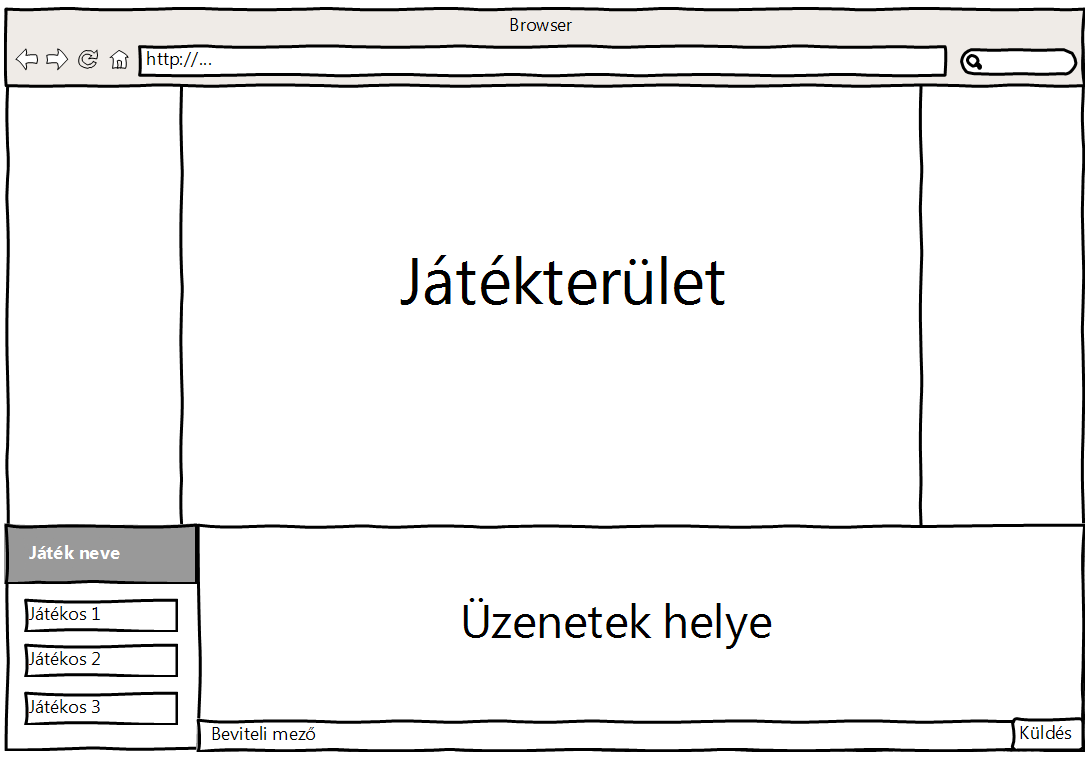
\includegraphics[scale=0.42]{media/image1.png}
\end{figure}

\section{Megvalósítás
előkészületei}


\subsection{Futtatókörnyezet
telepítése}

A választott futtatókörnyezet Node.js, ezt Windowson telepíthetjük a
nodejs.org-ról letölthető Windows Installer-el. Debian Linux
környezetben legkönnyebben parancssorból telepíthetjük az „\emph{apt-get
install nodejs}'' paranccsal. De akár portable (hordozható) változatot
is beszerezhetünk, ebben az esetben nincs szükség rendszergazda
jóváhagyására, de számolnunk kell apróbb kellemetlenségekkel.

A teszteléshez és a felület megvalósításához Mozilla Firefox-ot és
Google Chrome-ot is használok. Így biztosítani tudom, hogy mindkét
böngészőben minden zökkenőmentesen működik. Az internetezők több mint
60\%-a is e két böngésző egyikét használja.


\subsection{Fejlesztőkörnyezet
megválasztása}

A web fejlesztők többsége egyszerű szövegszerkesztőt használ a
fejlesztőmunka során. Windowson a legelterjedtebb a könnyen használható
Notepad++. Támogatja a szintakszis kiemelést és a forrásfájlok
automatikus formázására is van lehetőség. Hátránya, hogy csak
kezdetleges szókiegészítésre képes. Természetesen a feladat megoldására
teljesen alkalmas.

A szoftverfejlesztés során nem csak a forrásfájlokat szerkesztjük. A
program logikájának megvalósítását menet közben találjuk ki. Az így
megírt kódblokkok tesztelése természetes és szükséges. Előfordulnak
azonban összetett részfeladatok, amelyek elkészítése nem sikerül egyből.
A hibásan megírt program javítását hibakeresésnek vagy debugolásnak
hívjuk.


\subsubsection{A hibakeresés
módszere}

A hibakeresés során speciális hibakereső szoftvert használunk, amely
lehetővé teszi a program lépésenkénti futtatását, így képet kaphatunk a
program futásának bármely pillanatáról. Vizsgálhatjuk a változók
értékeit és a programot soronként léptethetjük, ezzel a hibák sokkal
könnyebben felderíthetőek, mintha csak egy hibás eredményt vagy
hibaüzenetet látnánk a program lefutása után.

Az általam választott platform is rendelkezik ilyen eszközökkel.
Legelterjedtebb a Node Inspector. Ez webes felületen engedi programunk
vizsgálatát. A mellékelt \ref{fejl} ábrán látható a Node Iinspector webes
felületének felépítése.
\begin{figure}[ht]
	\caption{Fejlesztőkörnyezet}
	\label{fejl}
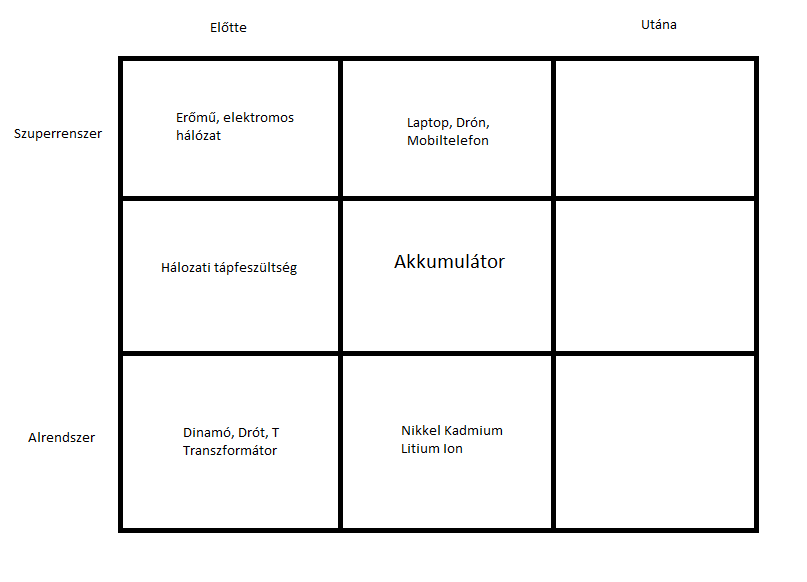
\includegraphics[scale=0.9]{media/image2.png}
\end{figure}


\subsubsection{Node Package Manager}

A Node.js egy tartozéka az „npm'', ami a Node.js csomagok telepítésére
és publikálására alkalmas. A sokféle probléma és az ezekre adott sokféle
megoldás kezelésére alkalmas ez. Egy csomag telepítése a „npm install
\textless{}csomagnév\textgreater{}'' paranccsal végezhető. A csomagok
telepítése történhet a központi adatbázisból, az internetről, vagy helyi
forrásból.


\subsection{Verziókövetés}

A szakdolgozat készítési folyamat egésze alatt verziókövetést használok.
Erre a legalkalmasabb a Git nevű verziókövető szoftver. Egyaránt képes
kis és nagy projektek kezelésére. A verziókövetés segít átlátni a
fejlesztések haladását, sorrendjét. A verziókövetés néhány egyszerű
műveletből áll. A szerkesztett fájlokat először kiválasztjuk, szakszóval
stage-eljük, majd amint elvégeztük a kívánt módosításokat és úgy
gondoljuk, hogy érdemes rögzíteni haladásunkat, véglegesítjük, más
szóval commit-oljuk az új verziót. Lehetőség van még új haladási szálak
létrehozására. Az így keletkezett ágakat a változtatások összesítésével
egyesíthetjük, így új verzió hozható létre. A kényelmi funkcionalitás
sem elhanyagolható. Egy parancs kiadásával továbbíthatjuk a helyi
változtatásokat egy központi tárolónak. A verziókezelés egyszemélyes
projekteknél nem kulcsfontosságú, de felgyorsítja és átláthatóvá teszi a
programfejlesztést.


\section{Megvalósítási
elképzelés}


\subsection{Modulokra bontás }

A program írása közben igyekeztem előre gondolkodni és minél
szakszerűbb, könnyen megérthető megoldásokat produkálni. Ennek a
tervezési folyamatnak során határoztam el, hogy külön fájlokat fogok
létrehozni a programegységeknek. Ez segíti az átláthatóságot és így a
szerkesztés folyamatát.

A moduláris programozás módszere szerint a programot különböző
függvényekre bontjuk. Ezek mindegyike egy pontosan meghatározott
feladatot lát el. Emellett az egyes programrészek a lehető legkevésbé
befolyásolják a program egészének működését és a programrészek egymással
való kapcsolatát. Ennek értelmében nem használunk vezérlőváltozókat.
Megfigyelhető még, hogy a függvények két nagy csoportot alkotnak. Egyik
a „vezérlők'' csoportja, a másik a „dolgozók'' csoportja. A vezérlők a
dolgozókat fogják össze, a dolgozók pedig kisebb részfeladatokat látnak
el.

A Node.js támogatja a moduláris programozást, tehát tartalmaz egy modul
betöltő rendszert. A modulok készítése egyszerű, csak az exports változó
egy attribútumába kell írnunk tetszőleges néven az elérni kívánt
függvényt, vagy értéket. Amennyiben egyetlen objektumot szeretnénk
exportálni, használhatjuk a module.exports változót, így nem kell
jellemzőnkként felépíteni az objektumot. Modulok betöltésére a require
függvényt használhatjuk, melynek első paramétereként a betölteni kívánt
fájl nevét kell megadnunk. Ez mind a Node.js jellegzetessége, tehát a
szabványos JavaScriptnek így a V8-nak sem szerves része.

Az én megvalósításom is ezekre alapul. A meghívott start program tölti
be a többi programrészt. Ez elegáns megoldás, hiszen könnyen
kezelhetjük, hogy mi töltődik be. Esetlegesen is csak a forrásfájlok
elejét kell szerkesztenünk, ha több vagy kevesebb modult szeretnénk
betölteni.


\subsection{Kapcsolatkezelő}

A kapcsolatkezelő a kiszolgálóarhiterktúra szélső eleme. Minden beérkező
csomag ezen halad át. Folyamatosan hallgat a megadott TCP porton. Új
kapcsolat esetén foglalkozik a kapcsolat felállításával és a felhasználó
mielőbbi kiszolgálásával. Üzenet esetén gondoskodik arról, hogy a
kiszolgáló egyéb érintett részei tudjanak a bejövő információról. Minden
bejövő kapcsolatot egy felhasználóhoz rendel. A kiszolgáló a
továbbiakban ez alapján könnyen tudja kezelni a kapcsolatokat. Fontos
szerepe van még kapcsolatok lezárásában is.


\subsection{Parancsértelmező}

A parancsértelmező a központi kiszolgáló és a kapcsolatkezelő közt
helyezkedik el. Minden olyan üzenet, ami a kapcsolatkezelőn túljut, a
parancsértelmezőbe kerül. A parancsértelmező feladata az üzenetek
feldolgozása, majd a döntés meghozatala. Parancsnak számít minden olyan
üzenet, ami per (/) jellel kezdődik. Ezek értelmezve vannak. Minden
egyéb üzenet felhasználói üzenetként jelenik meg.

Ez a modul a kiszolgáló vezérlője. Minden bekövetkező változás ide
vezethető vissza. Ha újabb feladatokat szeretnénk a kiszolgálóhoz
rendelni, akkor itt kell gondoskodnunk arról, hogy a megfelelő parancs a
kívánt programrészek lefutását eredményezze.


\subsection{Csoportkezelő}

A csoportkezelő a kiszolgáló magját képezi. A csatlakozó felhasználók
mindegyikéről tudomása van. Alapértelmezetten mindenki egy speciális
csoportba kerül. Innen indulva készíthetnek saját csoportot, vagy
csatlakozhatnak egy már létezőhöz.

A csoportok jelszóval védhetőek. Így csak a jelszót ismerő játékosok
tudnak csatlakozni. A jelszóval védett csoport ideális lehet például
ismerőseinkkel való beszélgetésre, mert így egyéb játékosok biztosan nem
fognak zavarni.

Minden csoportnak van egy tulajdonosa, aki jogosult azt átnevezni vagy
annak jelszavát megváltoztatni. Csoportot viszont a csoport tulajdonosa
sem szüntetheti meg. A csoport csak abban az esetben törlődik, ha azt
minden felhasználó elhagyta. Amennyiben a csoportot tulajdonosa
elhagyja, a csoport új tulajdonosa az első csatlakozott játékos lesz.


\subsection{Játékvezérlő}

A Játékvezérlő a programnak azon része, amely az egyes Játékok
lebonyolítását végzi. Egy-egy játékvezérlő rendelhető mindegyik
csoporthoz. A játékvezérlő már valós idejű technológiát alkalmaz, így
például képes követni minden egyes játékos nyomva tartott billentyűit és
erre közvetlen választ is képes küldeni. A játékvezérlő szintén
modulokból áll. A leglényegesebb a csatlakozó vagy távozó játékosok
kezelője, a játéklogika és a kliensek kiszolgálásáért felelős részek.


\subsection{A vezérlők közti
kommunikáció}

A vezérlők közti kommunikáció megtervezése igazi kihívásnak bizonyult.
Szem előtt tartottam a modulok hierarchiáját, és ehhez illesztettem a
kapcsolati sémát is, így bizonyos esetekben megspóroltam egy-egy
felesleges lépést. Ennek értelmében a vezérlők bizonyos műveleteiket egy
közös objektumon keresztül bonyolíthatják le. Ez sok extra munkát spórol
meg.

A vezérlők betöltésének sorrendje is kérdéses volt. Mivel a vezérlők
egymásra hivatkoznak, előfordulhat, hogy az egyik vezérlő a másik
betöltése előtt már szeretné azt használni. Erre megoldás, ha az egyes
modulok betöltése után megvárjuk, hogy az utolsó modul is betöltődjön.


\section{Fejlesztői
dokumentáció}

A megvalósítást a kiszolgáló oldalról közelítettem meg. A kiszolgáló a
központi egység, melynek minden körülménytől függetlenül működőképesnek
kell lennie. Tehát a kiszolgáló akkor is üzemel, ha nincs semmiféle
kapcsolat. A kezdeti fázisban pedig nincs is mi kapcsolódjon. Így a
kliens-oldal fejlesztése inkább a kiszolgáló teszteléseként alakul.

A fejlesztés egy sor tesztprogram megírásával kezdődött. A választott
technológiákat csak részben ismertem, így némi tapasztalatszerzésre volt
szükségem.


\subsection{WebSocket kapcsolat
felállítása}

A program kulcsfontosságú eleme a hálózati kapcsolat. A játék
működéséhez valós idejű kapcsolat szükséges. A választás a legtöbb
böngésző által támogatott WebSocket-re esett. Ez viszont nem minden. A
kiszolgáló megvalósításánál megválaszthatjuk, hogy melyik megvalósítást
használjuk. A választék széles, mindegyiknek megvannak a sajátosságai.


\subsubsection{A feladathoz megfelelő
megvalósítás}

A legelterjedtebbek a „ws'' és a „socket.io'', de említést érdemel még a
„faye'' és a „socketcluster''. Az utóbbira jellemző, hogy jelentősen
nagyobb teljesítményre képes társaihoz viszonyítva. Ezt az összes
processzormag kihasználásával éri el. Érdekes még a „primus''
megvalósítás. Ez az elérhető megvalósítások egy gyűjteménye, tartalmazza
az eddig említetteket és még néhány kevésbé ismertet is. Egyszerűen
válthatunk a megvalósítások között. Ezen kívül magában foglal néhány
sajátos fejlesztést is, így nagyobb stabilitást nyújt.

A választás ismét nehéz volt. A két kiemelkedő megvalósítás egyike a
''ws'', ami a leggyorsabb megvalósítás. Nagyságrendekkel gyorsabb, mint
a többi. A másik a „socket.io'', ami régebbi alternatív technológiákat
is támogat, így a régebbi böngészővel rendelkező felhasználók is
kapcsolódhatnak. A fejlesztési feladat szempontjából mindkettő fontos,
de én fontosabbnak tartottam, hogy a gyorsabb megoldást alkalmazzam, még
ha ez néhány felhasználónak kényelmetlenséget is okoz. Ezeket figyelembe
véve tehát a „ws''-el kezdtem kísérletezni.


\subsubsection{A kapcsolat tesztelése}

Az első kihívás a kapcsolat felállítása. Szerencsére példaprogram bőven
akad és a feladat sem nehéz. A „ws'' modul betöltése után példányosítjuk
azt. A kapott objektumhoz egy eseménykezelőt rendelünk. Ez a programrész
új kapcsolat fogadása esetén hívódik meg. Ezután a kapcsolathoz
rendelünk egy eseménykezelőt. Ez az egyes üzenetek érkezésekor hívódik
meg. Paraméterként megkapjuk az üzenetet is. A mellékelt példaprogram a
fogadott üzenetet kiírja, és válaszként az üzenetet csupa nagybetűvel
visszaküldi.

Ezt a programot könnyen tesztelhetjük is. Csak egy böngészőre van
szükségünk. A programrészt akár a fejlesztői parancssorba is
másolhatjuk.

Ha a kiszolgáló fut, akkor a kódban mutatott program sikeresen
kapcsolódik a helyi szerverhez, majd a „teszt üzenet''-et el is küldi. A
kiszolgáló ezt fogadja, kiírja, és csupa nagybetűvel visszaküldi. A
kliens ezt fogadja és feldob egy ablakot a „TESZT ÜZENET'' felirattal.
Tehát a kapcsolat működik, sőt annak mindkét oldalához logikát
rendelhetünk és az üzenetet fel is dolgozhatjuk.


\subsection{A kapcsolatok kezelése}


\subsubsection{Új kapcsolatok
adminisztrálása}

A kapcsolatok kialakítása megoldott, de ez még nem sok. A kapcsolatokat
azonosítani kell. Minden egyes kapcsolat új felhasználót hoz létre Az alábbi 
\ref{methods} táblázat alapján kell indítani a kérést. A
felhasználóhoz egyéb adatok is tartoznak, így például annak neve.

Az üzeneteket elküldés előtt megcímezzük. A címzett esetünkben nem a
kapcsolat, hanem egy felhasználó. A felhasználók mindegyike egy egyedi
azonosítóval rendelkezik. A felhasználókat azonosító alapján találjuk
meg. Az azonosító egy számlálóból származik. Ez gyakorlatban garantálja,
hogy nem lesz két felhasználó ugyanazzal az azonosítóval.

\begin{table}[ht]
	\centering
	\caption{HTTP metódusok}
	\label{methods}
	\begin{tabular}{|l|l|}
		\hline
		\rowcolor[HTML]{9B9B9B} 
		{\color[HTML]{000000} Metódus} & {\color[HTML]{000000} Jelentés} \\ \hline
		GET                            & Adat lekérése                   \\ \hline
		POST                           & Adat beszúrása                  \\ \hline
		PUT                            & Adat frissítése                 \\ \hline
		DELETE                         & Adat törlése                    \\ \hline
	\end{tabular}
\end{table}

\subsubsection{Kapcsolatzárás}

A kapcsolatkezelés része még a kapcsolatok lezárása. A kapcsolat
lezárása esetén, fontos hogy további adatcserére nincs lehetőség. Ez
problémát okoz abban az esetben, ha a kapcsolatot éppen üzenetküldés
közben zárjuk, vagy a kapcsolat lezárás nélkül megszakad. Az üzenet vége
már nem küldhető el. Ezt a kivételt kezelnünk kell. A hibát az alsóbb
protokollok adják, jellemzően azért, mert zárt kapcsolaton próbálunk
üzenetet küldeni, ami nem lehetséges. A kivétel kezelésére csak meg kell
hívnunk a kapcsolat zárása metódust. Ezzel ugyanaz az eredmény, mintha a
felhasználó szabályosan távozott volna a kapcsolat bezárásával.

A kapcsolat zárása fontos mozzanat a kiszolgáló részéről, hiszen azt
kezelni kell. Egy kapcsolat bezárásával egy felhasználó távozik. Ekkor
körültekintően kell eljárni, biztosítani kell, hogy a felhasználó
távozásáról értesüljön minden érintett részprogram. Ebben az esetben
csak a csoportkezelő, mert a további intézkedések erre vannak bízva.


\subsubsection{Üzenetfogadás}

A kapcsolatkezelés része még a beérkező üzenetek irányítása is. Az
üzenetek értelmezését a parancsértelmező végzi, így hát a beérkező
üzeneteket a parancsértelmező kapja meg. Az üzenet mellett szerepel a
küldő is. Ez igen fontos, mivel tudnunk kell, hogy melyik parancsot
melyik felhasználó küldte. Ezután az üzenettel a kapcsolatkezelő nem
foglalkozik.


\subsubsection{Üzenetküldés}

A kapcsolatkezelő még egy dologról gondoskodik, ez pedig a kimenő
üzenetek. Minden kimenő üzenet egy felhasználónak van címezve. Ez az
üzenet a felhasználóhoz rendelt kapcsolaton fog célba érni. A program
bármely ponton küldhet üzenetet a kliens felé. Ehhez csupán egy
felhasználó objektumra lesz szükség.


\subsection{A parancsértelmező}

A parancsok mit sem érnek, ha nincsenek végrehajtva. A parancsértelmező
gondoskodik arról, hogy a felhaszanáló által kiadott parancs a felelős
modulhoz jusson, a megfelelő paraméterekkel. Lényegében csak parancsok
szintaxisát rendeli programrészekhez.

A kapott üzenetekről először eldönti, hogy parancs vagy felhasználói
üzenet-e. Ha parancs, akkor először az üzenetet darabokra vágja a
megadott elválasztó karaktereknél. Az így kapott tömböt elemenként már
ki lehet értékelni.

Az érintett modul kiválasztása az első. Ez lehet a csoportkezelő, vagy a
játékvezérlő. Majd következik a parancs kiválasztása. A csoportkezelőnek
legfontosabb utasításai a csoport létrehozása, a csoportba lépés, a
csoport elhagyás, a létező csoportok listázása és egy adott csoport
adatainak lekérése. Ezek közül néhányat csak paraméterrel lehet
meghívni.


\subsection{A csoportkezelő}

A csoportkezelő, mint már említettem központi része a kiszolgálónak.
Fontos feladatot lát el, a kapcsolatkezelőtől és a parancsértelmezőtől
is utasításokat fogad el. Kezdeti állapotban is létezik egy speciális
szoba, a nulladik szoba. A nulladik szoba a modul betöltésekor jön
létre. A kapcsolatkezelő minden új kapcsolat esetén ebbe a csoportba
helyezi az újonnan létrejött felhasználót.


\subsubsection{Csoportok
létrehozása}

A kapcsolódó felhasználók a megfelelő paranccsal hozhatnak létre szobát.
A parancsot a parancsértelmező kapja meg és értelmezi. Megfelelő parancs
esetén kérést küld a csoportkezelőnek, ami teljesíti az utasítást. A
szoba létrehozás parancsnak megadható a létrehozni kívánt szoba neve,
ezt nem kötelező megadni. Ha nincs megadva név, akkor a szoba neve a
szerveren beállított módon a csoportot létrehozó játékos nevéből
generálódik.


\subsubsection{Csoportba lépés
menete}

A felhasználó a megfelelő parancs kiadásával csoportba léphet. A
csoportba lépés több mozzanatra osztható.

Csoportba lépés feltételei

Akárki akármikor megpróbálhat tetszőleges csoportba csatlakozni. Ennek
két kimenetele lehet. Az egyik, hogy sikerül a szobaváltás, így a
felhasználó kérése teljesült. A másik, hogy a kérés végrehajtása
megszakad. Ennek több oka is lehet. A szobába lépés nem történhet meg,
ha a felhasználó egy nem létező szobába próbál csatlakozni, vagy akkor,
ha a csoport jelszóval védett és a megadott jelszó helytelen. A
meghiúsult végrehajtás hibaüzenettel jár, amit a felhasználó meg is kap.
A parancs kiadásának így semmi hatása nincs. A felhasználó marad az
eredeti csoportjában.

Sikeres csoportváltás lépései

Ideális esetben a csoportváltás sikeres. Először a felhasználó lekerül a
csoport tagjait tartalmazó listáról. Ilyenkor a felhasználó eredeti
csoportjának tagjai kapnak egy üzenetet arról, hogy a megadott
felhasználó elhagyta a szobát, tehát innentől ő nem kapja meg a szoba
üzeneteit.

Az új csoportba lépésnél a célcsoportban lévő felhasználók listájára
kerül az új tag. Emellett a célszoba tagjai kapnak egy üzenetet arról,
hogy az adott felhasználó csatlakozott és már ő is „hallja'' a
beszélgetést.


\subsubsection{Csoport elhagyásának
menete}

A csoport elhagyására is van lehetőség. A szoba elhagyása a
csatlakozáshoz hasonló. Az eredeti szoba listájából törlődik a
felhasználó, az új szoba listájába pedig belekerül. Emellett mindkét
csoport tagjai megkapják a megfelelő értesítést. Egyébként ez
egyenértékű a nulladik szobába való csatlakozással, ezért gyakorlatban
ez így van megoldva.


\subsubsection{Üres szobák
kezelése}

Egy szoba megüresedik, hogyha minden felhasználó elhagyja azt. Itt
elhagyás alatt értjük a másik szobába csatlakozást is. Az üres szobák
felhalmozódását tehát meg kell előzni. Erre az a megoldás született,
hogy ha a szobát az utolsó felhasználó is elhagyja, a szoba megszűnik.


\subsubsection{Segédfüggvények}

A szobakezelő több segédfüggvényt is tartalmaz, ezek nem feltétlenül
szükségesek a szobakezelés működéséhez, de logikailag ide tartoznak.
Ilyen függvény például a csoportok listázása, vagy a csoportos
üzenetküldés. A modul tartalmaz segédmetódusokat, de a legtöbb kívülről
is elérhető.


\subsubsection{Hívható
függvények}

A kiszolgáló minden részprogramjából elérhető hívások ezek. Egy zárt
egységet, ebben az esetben a szobakezelőt rejtik maguk mögött. Csak
korlátozott hozzáférést engednek, pontosabban csak az előre megszabott
utasításokat hajtják végre. A helyi változókkal és a felhasználók
kezelésével a hívó programrésznek nem kell foglalkoznia. Például csak
annyit kell mondanunk, hogy az adott felhasználót az adott szobába
szeretnénk rakni. Ezzel mi végeztünk is a feladattal. A csoportkezelő
majd gondoskodik annak elvégzéséről.

Ez a megoldás követi az objektumorientált programozás adatrejtés elvét,
ami szerint az adattagok alapesetben védettek, és csak a szükséges
adattagok érhetőek el. Az elérés közvetlen elérés helyett jellemzőkkel
van megoldva.

A JavaScript nyelvben lehetőség van jellemzők létrehozására, Ez viszont
más nyelvekhez képes jelentősen kényelmetlenebb.

A kód mutatja a csoportkezelő egyik jellemzőjének létrehozását.
Ennek első lépése az elérni kívánt függvény létrehozása. Ezután az
„Object.definePorperty'' metódussal készíthető el a kívánt jellemző. Az
első paraméter a módosítani kívánt objektum, a végrehajtás után ennek az
objektumnak lesz tagja a jellemző. Az új attribútum neve a második
paraméterként megadott változó értéke lesz. A harmadik paraméterben
pedig egy asszociatív tömbben adhatjuk meg jellemző leírását. A leírás
határozza meg, hogy mi történjen a jellemző írásakor, olvasásakor vagy
meghívásakor. Ezen felül megadhatjuk, hogy a jellemző felülírható-e.


\subsection{A játékkezelő}

Minden csoporthoz alapértelmezetten egy játékkezelő is tartozik. A
játékkezelő kezdetben nem aktív, de már ebben a passzív állapotban is
fontos szerepe van. A játékkezelőnek mindig készen kell állnia a játék
elindítására, ezért már a kezdettől figyelemmel kíséri a szobába lépő és
azt elhagyó játékosokat.


\subsubsection{Játékba lépés}

Ahogy a felhasználó játékba lép, azt játékosként is kell adminisztrálni.
A játékosokhoz nem csak a névvel, azonosítóval és a kapcsolattal
ellátott felhasználói adatstruktúra tartozik. A játékos lehet csapat
tagja, rendelkezhet pontszámmal és még sok más a játéktípustól függő
változóval. A játékosok jellemzőit csatlakozáskor alaphelyzetbe kell
állítani. Ezeket a tulajdonságokat részben a játék határozza meg. A
játékmenet jórészt ezen értéktől függ.

A játékosok jellemzői

A játékos jellemzői egy játékos objektum attribútumaiként vannak
tárolva. A játékos első attribútuma annak típusa. Alapesetben játékos,
de ennek szerepe, hogy a részprogramok is tudhassák, hogy a kérdéses
objektum játékos. A második jellemzője a játékosoknak a felhasználó. Ez
a felhasználó típusú objektum lehetővé teszi az egyedi azonosítást és a
közvetlen üzenetküldést. A játékkezelő a játékos nevének a felhasználó
nevét használja.

Ezután a játékra jellemző attribútumok következnek. Így a játékos
csapata, a játékos pontszáma, pozíciója, sebessége, mérete. Követve
vannak még a játékos lenyomott gombjai is, és az utolsó kiküldött
frissítés adatai is.


\subsubsection{Játék elhagyása}

A játék elhagyásának kezelése egy újabb feladat. Ennek során a játékost
ismét csak el kell távolítani a csapatból, de itt már egészen más
dolgokkal is kell foglalkozni. Itt már a játék logikájától függően kell
eljárni. Esetünkben a felhasználó pontszámát nullázni kell, és ha
esetleg a játékosnál zászló van, akkor annak is vissza kell kerülnie a
helyére.


\subsubsection{A játék
elindítása}

A játék a start metódus hívásával indítható el. A játék ekkor végzi el
az utolsó előkészületeket, betölti a pályaelemeket, többek között a
zászlókat és a pályán lévő akadályokat. A játék ekkor még mindig nem
indulhat el. A indulás előtt a játékelemeket még inicializálni kell. Ezt
egyetlen függvény végzi. A függvény a játékelem típusától függően végzi
el az összes szükséges beállítást. A játék elindításával a játék
státusza „running''-ra vált. Ezzel jelzi, hogy a játék elkezdődött. A
játék most már valóban készen áll a működésre.


\subsubsection{A játék futása}

A játék menete a játék folyamatos frissítéséből származik. Ez a
frissítés ideális esetben fix időközönként következik be. Minden
frissítés alkalmával lefut a játék frissítésére szolgáló logika. A
logikában van meghatározva, hogy a játék hogyan reagál egyes
helyzetekre, például a megfelelő gomb lenyomása esetén a játékos
mozgásba lendül. Ha a mozgás hatására beleütközik valamibe, akkor
visszapattan. A játéklogika efféle esetek feldolgozásából áll.

A játék futása tehát a frissítéseknek köszönhető. A frissítési
programrészt pontos időközönként kell meghívni. Erről a játék
elindításakor létrehozott időzítő gondoskodik.


\subsubsection{A játék
frissítése}

A JavaScript alapértelmezetten támogatja az időzítőket. A mellékelt kódban
látható ennek működése. A „timer'' a játék egy belső objektuma. A
„setInterval'' függvénnyel időzítőt készíthetünk, amely tetszőleges
függvényt hív meg tetszőleges időközönként. Esetünkben a játék
frissítésére szolgáló „update'' metódust 10 milliszekundumonként, tehát
másodpercenként 100-szor. Minél kisebb a frissítések között eltelt idő,
annál folyamatosabb lesz a játék. Ennek persze határt szab a számítás és
a megjelenítés teljesítménye is. A számítási sebesség nem gond,
gyakorlatilag csak a megjelenítés sebessége szab határt. A forgalomban
lévő monitorok frissítési sebessége korlátozott, jellemzően 60 hertz. Ez
annyit jelent, hogy a kép másodpercenként 60-szor frissül. Ez jelentősen
kevesebb, mint a játékfrissítés sebessége. Ennek eredménye, hogy a
megjelenítés nem fogja a játék minden állapotát ábrázolni. Előfordul
majd, hogy képkockák között két frissítési ciklus is lefut. Játékoknál
ez gyakran előfordul, ennek a frissítési eltérésnek nincs szemmel
látható következménye.


\subsubsection{A játék lezárása}

A játék játékos nélkül nem létezhet. Ezért ha az utolsó felhasználó is
elhagyja a játékot, a játék véget ér. A játék frissítését le kell
állítani. Ezt, a már korábban mutatott „timer'' objektum segítségével
tehetjük meg. Pontosabban ennek elnevezésére és tárolására csak azért
volt szükség, hogy azt később törölhessük. Ha nem mentettük volna el,
akkor most nem tudnánk törölni azt. Az időzítő funkciók egyébként
globális objektumként érhetőek el, tehát a „require'' használata nélkül.


\subsubsection{A játéküzenetek}

A játékkezelőnek fontos, hogy a felsőbb utasításokat fogadni tudja. Erre
a „message'' metódus ad megoldást. A játéknak a kiszolgálóprogram
akármelyik részprogramja küldhet üzenetet. Ezek az üzenetek
felhasználóhoz kötöttek. Az üzenetek itt ismét értelmezésre kerülhetnek,
ezt már a játéklogika határozza meg. Valójában a megvalósításban ezek az
üzenetek csak a felhasználó által megnyomott billentyűk kezelésére
vannak használva, így ezek az üzenetek nincsenek valójában lekezelve.


\subsection{A játékmotor}


\subsubsection{A játékmotor célja}

A játékmotor nem más, mint a játékötlet megvalósításának a
keretrendszere. A játékmotor megoldásokat biztosít az elemi műveletek
végrehajtásához. A játékmotor jól illeszkedik az eddigi rendszerbe. A
játékmotor valójában a játékkezelő része. Egységes módon enged
interakciót a felhasználói felülettel. Ez a már elkészült
programrészeken nyugszik. Az üzenetek elküldése a már jól bevált módon
zajlik. Kérdéses viszont, hogy az elküldött adatot hogyan ábrázoljuk a
felhasználói oldalon. Ennek megoldása a kliens-oldali
parancsfeldolgozás. A kliens megkapja a rá vonatkozó utasításokat, egy
objektumstruktúrában. Ezt feldolgozva megkapja, hogy milyen objektumokat
kell megjeleníteni.


\subsubsection{A játék lehetséges
elemei}

A játékhoz csak néhány elemre van szükség. Ezek mindegyike meghatározott
tulajdonságokkal bír. Legfontosabbak a zászlók. Ezeknek egyik jellemzője
a tulajdonos csapat azonosítója. Játékelemek még a játékban lévő falak,
körök és egyéb akadályok. Ezek mindegyike eltérő módon van kezelve mind
a szerver, mind a kliens oldalán. De fontos, hogy a játék a \ref{spec} pontban említetteknek megfeleljen.


\subsubsection{Megjelenítés a
kliens-oldalon}

Az egyes elemekhez más-más megjelenítési procedúra van rendelve.
Általánosan igaz, hogy az elemeknek van pozíciója, és valamiféle
kiterjedése. A vonalak kezdő és végpontjukkal vannak megadva. A köröknek
pozíciója és sugara van. A szövegnek pozíciója, értéke és mérete is van.
A most felsoroltak mindegyikének megadhatunk színt is. Vannak még
speciális jellemzők is, ezek egyike alkalmas a szöveg középre
igazítására. A megjelenítendő adathalmaz tartalmaz még egy pozíció
típusú bejegyzést is. Ez az adott játékos pozícióját jelöli a pályán.
Ennek ismeretében megoldható, hogy a „kamera'' kövesse a játékost. A
követés gyakorlatilag csak annyit jelent, hogy minden el van csúsztatva
ezzel a pozícióval.

Lehetőség van még közvetlenül a felületre rajzolni. Ekkor a követett
játékos pozíciója nem befolyásolja a megjelenítést.


\subsubsection{Játékobjektumok}

A választott zászlójátékban lényeges, hogy a játékosok a pálya mely
részeire juthatnak el. Erről a játéklogikában kezelt objektumok
listájának megfelelő értelmezése és az azokból származó szabályok
betartása gondoskodik. A listában szereplő minden egységnek megvan a
sajátos viselkedése. Ez a játék minden frissítési lépésénél lefut és
kifejti hatását a többi játékelemre, így befolyásolva a játék további
menetét.


\subsubsection{Rugalmas ütközés}

A játék működéséhez kulcsfontosságú az ütközések helyes kezelése. A
rugalmas ütküzés pontos szimulálását kellett megoldanom. Természetesen
itt érvényes az energiamegmaradás törvénye, tehát az ütközés során
mozgási energia el nem vész, csak áttevődik. A játékban az objektumok
kölcsönhatására általánosan igaz ez.


\subsubsection{Ütközés fallal}

A legegyszerűbb és leggyakoribb játékelem a fal. A falak a már említett
módon, játékobjektumként vannak kezelve. A fal logikája kimondja, hogy
mi történik, ha egy játékos falnak ütközik. A logika első lépése a
tesztelés. Meg kell bizonyosodni arról, hogy a játékos ütközött. Ha
ennek a vizsgálatnak az az eredménye, hogy a játékos ütközött, akkor azt
kezelni kell. Az ütközés kezeléséhez át kell gondolni, hogy hogyan is
ütközött az elem és hogy mi a várt eredmény.

\begin{figure}[ht]
	\caption{A mozgásvektor számítása}
	\label{kor:mozg}
	\tikzset{every picture/.style={line width=0.75pt}} %set default line width to 0.75pt        
	
	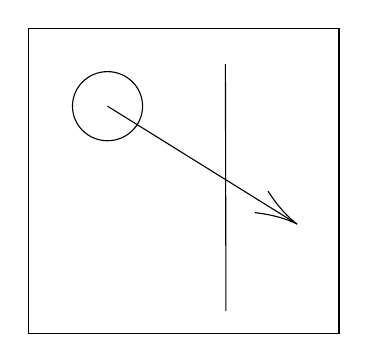
\begin{tikzpicture}[x=0.75pt,y=0.75pt,yscale=-1.85,xscale=1.85]
	%uncomment if require: \path (0,300); %set diagram left start at 0, and has height of 300
	
	\draw    (99.83, 79.5) rectangle (180.75, 159)   ;
	\draw    (120.48,99.8) -- (169.83,130.5) ;
	\draw [shift={(169.83,130.5)}, rotate = 211.89] [color={rgb, 255:red, 0; green, 0; blue, 0 }  ]   (0,0) .. controls (3.31,-0.3) and (6.95,-1.4) .. (10.93,-3.29)(0,0) .. controls (3.31,0.3) and (6.95,1.4) .. (10.93,3.29)   ;
	
	\draw    (120.48, 99.8) circle [x radius= 9.13, y radius= 9]  ;
	\draw    (151.18,88.85) -- (151.32,153.15) ;
	
	
	\end{tikzpicture}
	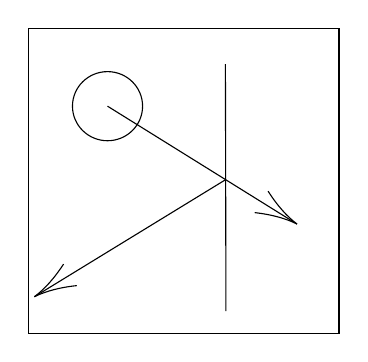
\begin{tikzpicture}[x=0.75pt,y=0.75pt,yscale=-1.85,xscale=1.85]
	%uncomment if require: \path (0,300); %set diagram left start at 0, and has height of 300
	
	\draw    (99.83, 79.5) rectangle (180.75, 159)   ;
	\draw    (120.48,99.8) -- (169.83,130.5) ;
	\draw [shift={(169.83,130.5)}, rotate = 211.89] [color={rgb, 255:red, 0; green, 0; blue, 0 }  ]   (0,0) .. controls (3.31,-0.3) and (6.95,-1.4) .. (10.93,-3.29)(0,0) .. controls (3.31,0.3) and (6.95,1.4) .. (10.93,3.29)   ;
	
	\draw    (120.48, 99.8) circle [x radius= 9.13, y radius= 9]  ;
	\draw    (151.18,88.85) -- (151.32,153.15) ;
	
	
	\draw    (151.07,119.04) -- (101.43,149.43) ;
	\draw [shift={(101.43,149.43)}, rotate = 328.53] [color={rgb, 255:red, 0; green, 0; blue, 0 }  ]   (0,0) .. controls (3.31,-0.3) and (6.95,-1.4) .. (10.93,-3.29)(0,0) .. controls (3.31,0.3) and (6.95,1.4) .. (10.93,3.29)   ;
	
	
	\end{tikzpicture}
	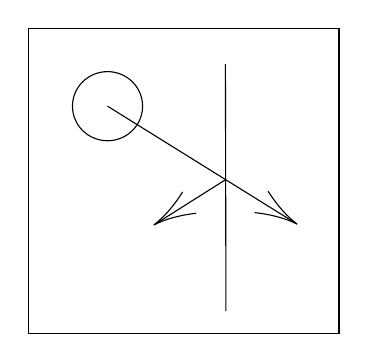
\begin{tikzpicture}[x=0.75pt,y=0.75pt,yscale=-1.85,xscale=1.85]
	%uncomment if require: \path (0,300); %set diagram left start at 0, and has height of 300
	
	\draw    (99.83, 79.5) rectangle (180.75, 159)   ;
	\draw    (120.48,99.8) -- (169.83,130.5) ;
	\draw [shift={(169.83,130.5)}, rotate = 211.89] [color={rgb, 255:red, 0; green, 0; blue, 0 }  ]   (0,0) .. controls (3.31,-0.3) and (6.95,-1.4) .. (10.93,-3.29)(0,0) .. controls (3.31,0.3) and (6.95,1.4) .. (10.93,3.29)   ;
	
	\draw    (120.48, 99.8) circle [x radius= 9.13, y radius= 9]  ;
	\draw    (151.18,88.85) -- (151.32,153.15) ;
	
	
	\draw    (151.07,119.04) -- (132.56,130.73) ;
	\draw [shift={(132.56,130.73)}, rotate = 327.74] [color={rgb, 255:red, 0; green, 0; blue, 0 }  ]   (0,0) .. controls (3.31,-0.3) and (6.95,-1.4) .. (10.93,-3.29)(0,0) .. controls (3.31,0.3) and (6.95,1.4) .. (10.93,3.29)   ;
	
	
	\end{tikzpicture}
\end{figure}

A \ref{kor:mozg} ábrán a pontszerű ütközés számításának lépéseit lehet nyomon
követni. Elsőként azt kell észrevenni, hogy ütközés fog bekövetkezni.
Ütközés akkor következik be, ha egy mozgó objektum útjában egy másik
objektum áll. A \ref{kor:mozg} ábrának az első lépésében láthatjuk, hogy az
irányvektor metszi a falat. Ennek a feltételnek a bekövetkezésekor fut
le a visszapattanás logikája. Ez kiszámolja, hogy az új vektor merre
mutat. Ezt a \ref{kor:mozg} ábra második lépése mutatja. Itt látszik a mozgó test
ütközés utáni irányvektora is. A harmadik lépés pedig a játékelem
ütközés utáni pozícióját mutatja. Ezt az ütközési felületen „túllógó''
vektor ütközési felületre való tükrözésével kapjuk meg.

A pontszerű test ütközésekor a test elmozdulási irányvektorának az egyik
komponense megfordul, a beesési és visszapattanási szög pedig
megegyezik. A pontszerű ütközés könnyen alakítható kiterjedéssel
rendelkező kör ütközésévé úgy, hogy a falat a kör sugarával eltoljuk.
Ezt mindkét irányból meg kell tenni. A falaknak van eleje és vége is. Az
eddig mutatott metódus ezt nem kezeli, így a mozgó test a fal végén
„belemehet'' abba. Ennek egyszerű megoldása, hogy a falak végeit egy
apró körrel zárjuk, így a mozgó kör majd ezekkel fog ütközni. Ez
egyszerű megoldás, hiszen úgyis szükséges a kör-kör ütközés
megvalósítása.


\subsubsection{Ütközés körrel}

Körök ütközésekor azok közül legalább az egyiknek mozgásban kell lennie.
Az ilyen ütközést és kimenetelét átgondolni is bonyolultabb, így azt
leprogramozni is nehezebb, mint a fallal történő ütközést.

Közvetlen ütközés során a mozgásban lévő egységek mozgási energiája
megmarad, áttevődik. Ahogyan a \ref{kor:utk} ábra is mutaja, ha egy 
álló testnek ütközik valami, akkor az addig
álló test mozgásba lendül és az addig mozgó test megáll. Amennyiben egy
lassan mozgó testet hátulról egy gyorsabban mozgó test löki meg, akkor
az ütközés után az első test gyorsabban, a hátsó test lassabban fog
mozogni. Így gyakorlatilag megcserélődik a mozgások irányvektora.


\begin{figure}[ht]
	\caption{Az eltrítési szög kiszámítása}
	\label{kepletcsoport}
	\begin{eqnarray}
	\label{eq:group_first}
	\gamma_v & = & atan2(y_{21}, x_{21}) \\
	\label{eq:group_second}
	\gamma & = & \gamma_{xv} - \gamma_v \\
	r_d & = & d \cdot sin(\gamma)/r_{12} \\
	\alpha & = & sin(r_d)
	\end{eqnarray}

\end{figure}

Egy másik, problémásabb eset, amikor a testek csak „súrolják'' egymást.
Ilyenkor az ütközés után a testek mozgásának vektora kiesik az ütközési
síkra merőleges egyenesből. Ennek kiszámításához hasznos \ref{eq:group_first}-ben használt
 atan2 függvény. A következő lépésben a kapott szöget kivonjuk az irányvektorból. Ez látható \ref{eq:group_second} sorban.

\begin{figure}[ht]
	\caption{Kör-kör ütközés}
	\label{kor:utk}
	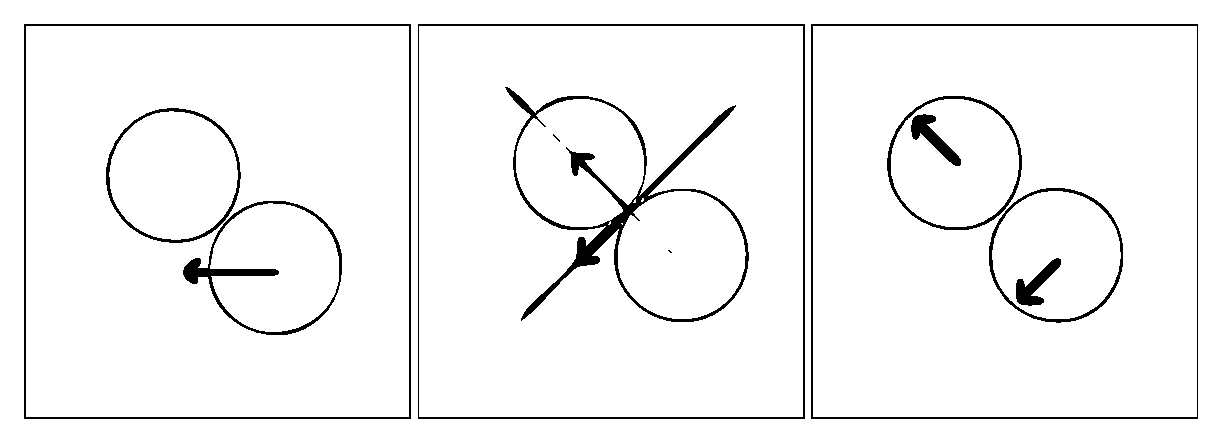
\includegraphics[scale=0.6]{media/image8.eps}
\end{figure}

A helyes értékek kiszámításához az irányvektorokat az ütközési sík és az
arra merőleges egyenes komponenseiként kell felírni, majd az ütközési
síkra merőleges komponenseket felcserélni. Ez a legegyszerűbb módszer.
Az algoritmus csak tökéletesen rugalmas ütközés szimulálására képes és
különböző tömegű testeket sem kezel.


\subsubsection{Ütközés
játékossal}

Játékosok ütközése során a játékfizika szempontjából kör-kör ütközésről
beszélhetünk. Ilyenkor mindkét játékos mozgásban lehet, így az ütközés
gyakorlati megvalósítása igazi kihívássá válik. A már bemutatott
klasszikus ütközés első megvalósítási kísérlete nem hozott sok sikert.
Némi kutatás után több eltérő megoldást is találtam.
\begin{figure}[ht]
	\caption{Sebesség ütközés után, tömegtől függően}
	\label{keplet}
\begin{equation}
\label{eq:single}
v_1=\frac{u_1\cdot (m_1 - m_2) + 2m_2 u_2}{m_1 + m_2} 
v_2=\frac{u_2\cdot (m_2 - m_1) + 2m_1 u_1}{m_1 + m_2}
\end{equation}

\end{figure}


A saját algoritmus hibáit a \ref{eq:single} képlet alapján javítottam, így már tökéletesen
működik, és tetszőleges számú játékos esetén is jó. A játékosok
ütközésének kezelésébe bele kellett építeni a zászlók kezelését is.


\subsubsection{Pontszerzés és annak
logikája}

A zászlószerzés a játék központi célja. Ezek kezelése összeolvad a játék
fizikai számításaival. A programban zászlók is speciális körként
jelennek meg. A zászló felvétele az inRange függvénynek köszönhető. Ez
dönti el, hogy a körök összeérnek-e. A zászló elvétele ugyanígy működik.


\section{Felhasználói
dokumentáció}

A játék böngészőből játszható. A játékhoz az tud csatlakozni, aki ismeri
a címet, amin a játékba be lehet lépni. A játékhoz kapcsolódás menete a
játék üzemeltetőjétől függhet. Általában a játékba be lehet lépni az
üzemeltető webcímét felkeresve, de előfordulhat, hogy az üzemeltető nem
rendelkezik webcímmel. Ebben az esetben az üzemeltető IP címét
felkeresve is csatlakozhatunk a játékhoz. A harmadik eshetőség, hogy a
kapcsolódáshoz szükséges fájlokat manuálisan kell beszerezni. Ez csak
erősen korlátozott elérésű hálózatnál szükséges.


\begin{figure}[ht]
	\caption{Lobby}
	\label{lobby}
	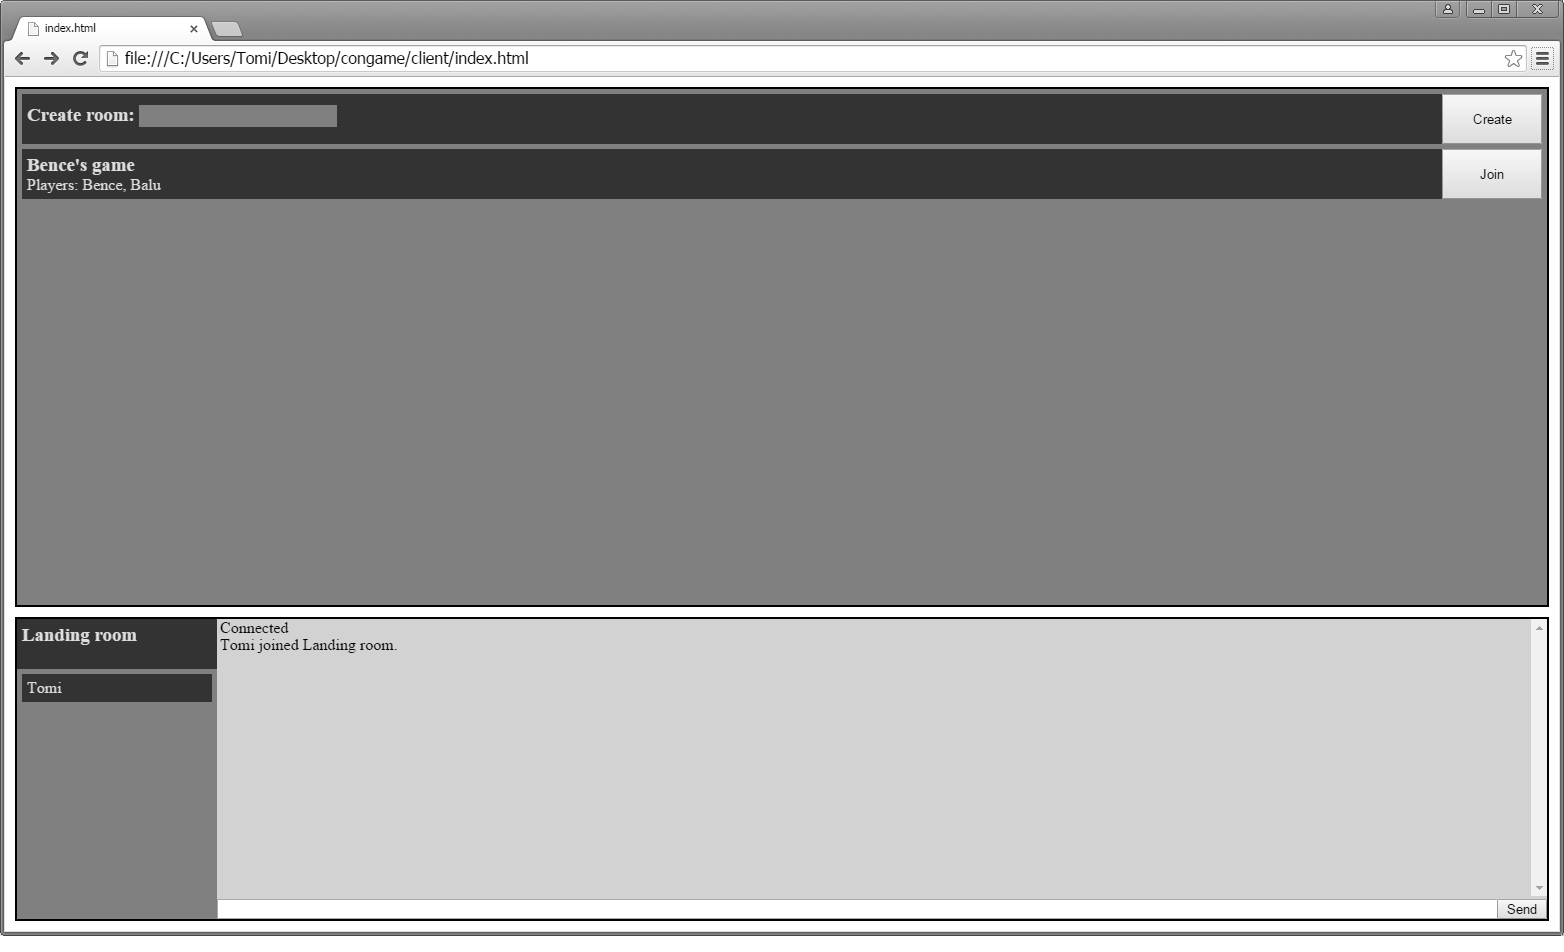
\includegraphics[scale=0.29]{media/image10.png}
\end{figure}



Sikeres kapcsolat esetén betöltődnek az oldal interaktív részei is. Ezt
követően egészen a kapcsolat bontásáig lehetőségünk van üzeneteket
küldeni. Az üzeneteket mindig csak az aktuális szoba felhasználói kapják
meg. Belépés után mindenki az úgynevezett előszobába kerül. Innen már
minden funkció egy kattintásnyira van. A felhasználói felület központi
részén jelenik meg a fő tartalom. A \ref{lobby} ábrán látható, hogy az
előszobában listázva vannak az elérhető szobák. A szobákba a jobb
oldalon lévő gombbal léphetünk. A felső gombbal saját szobát nyithatunk.
A szobának a nevét bal oldali szövegdobozba írhatjuk.

A felhasználói felület másik jelentős eleme az alsó üzent doboz. Ennek
bal oldalán a szoba neve és játékosai látszódnak. Játék közben egyéb
információk is megjelennek itt, pl. a játékosok pontszáma. Az alsó
szövegdobozba lehet üzeneteket írni. Az üzenet Enter-el vagy a küldés
gombbal továbbítható.

Új szoba készítésekor a készítő rögtön a játékba kerül. A pályán
mozoghat, gyakorolhat, amíg a meccs el nem kezdődik. A játszma akkor
indul, ha a játékosok többsége készen áll a küzdelemre.

A \ref{game} ábrán látható maga a játék. A csapatok összesített pontszáma
felül, baloldalon alul pedig a játékosokra lebontva látható a szerzett
pontok száma. A baloldali információs fülön megjelenik még egy kilépés
gomb is. Ezzel a felhasználó elhagyhatja a szobát.

A játék irányítása a nyíl gombokkal, vagy a WASD gombokkal történhet. Az
irányításhoz a játékterületnek kell aktívnak lennie. A meccsel
kapcsolatos további információkat a TAB gomb lenyomásával érhetjük el.

A játékból kilépéshez nem kell mást tenni, csak a böngészőablakot
becsukni.

\begin{figure}[ht]
	\caption{A játék}
	\label{game}
	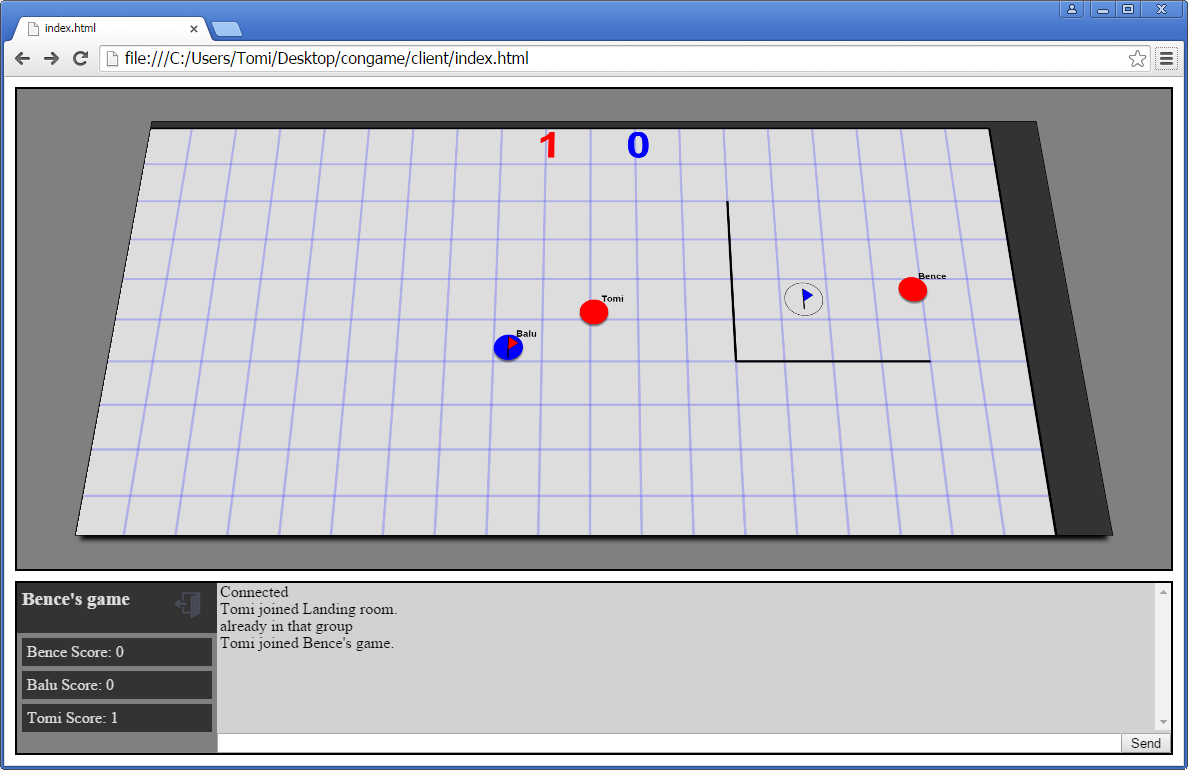
\includegraphics[scale=0.385]{media/image11.png}
\end{figure}


\section{Telepítés, üzembe
helyezés}

A program üzembe helyezése kifejezetten egyszerű. A Node.js-ben írt
programokat nem kell fordítani, ezért elég csak a forrásfájlokat
megszerezni. A támogatott operációs rendszerek mindegyikén a node
futtatható állományt kell meghívni a futtatni kívánt forrás fájlal. Ez a
program már képes további forrásfájlok, modulok betöltésére.

Az üzembe helyezés legfontosabb pontja a Node.js futtatókörnyezet
telepítése. Ez a telepítés mindegyik platformon máshogyan történik.
Általánosan jellemző, hogy rendszergazda jogosultságra van szükség a
teljes telepítéshez.

A Node.js Windows rendszerre a nodejs.org/downloads-ról letölthető .exe
és .msi telepítő csomag formában is. Amennyiben rendszergazda joggal nem
rendelkezünk, akkor ezek egyikének sem vesszük hasznát. Az
alapértelmezett beállításokkal való telepítés után a
C:\textbackslash{}Program Files (x86)\textbackslash{}nodejs mappában
találjuk a futtatókörnyezet fájljait, így egy node.exe-t is. A
programunk futtatásához ezt a programot kell, meghívni a megfelelő
fájlal.

Debian rendszeren valamivel egyszerűbb a telepítés. A központi tárolóból
közvetlenül telepíthető a „nodejs'' nevű csomag. A telepítéshez ismét
szükséges rendszergazda jogosultság.

Mac OS X rendszeren a telepítés nodejs.org/downloads-ról letölthető .pkg
csomaggal a legegyszerűbb. Ennek telepítéséhez ismét szükséges
rendszergazda jóváhagyása. A telepítés után már egyik platformon sem
szükséges adminisztrátori engedély.

A program futása a beállításoktól függően igényelhet speciális
engedélyét. A kiemelt portok lefoglalása általában rendszergazda joghoz
kötött.

Ha ezeket az akadályokat sikerül elhárítani, akkor már semmi akadálya,
hogy a program megfelelően működjön. A program a start.sh futtatásával,
vagy a „node start.js'' parancs kiadásával futtatható.


\section{Összefoglalás}

A szakdolgozatomban egy ügyességi játék megvalósítását tűztem ki célul.
Végig fontosnak tartottam, hogy ésszerű irányba haladjon a fejlesztés.
Fontosnak tartottam még azt is, hogy a lehető legalacsonyabbak legyenek
a környezettel kapcsolatos elvárások. Ily módon minden modern operációs
rendszer és böngésző képes az általam írt program futtatására.

A program minden részét JavaScript nyelven írtam. Eleinte alig ismertem
a technológiát, a fejlesztés során viszont megbarátkoztam a számomra új
nyelvezettel. Mára mondhatom, hogy ismerem a JavaScript-et és biztos
vagyok benne, hogy ennek még később is hasznát veszem. Visszatekintve
büszkeséggel tölt el, hogy így bele mertem vágni egy addig ismeretlen
témába.

Hiszem, hogy értéket alkottam, és remélem, hogy sokaknak lesz lehetősége
kipróbálni a játékomat. Számomra a játék létrehozásának minden lépése
örömet szerzett.


\nocite{*}

\let\oldsection\section
\let\Section\section 
\def\section*#1{\Section{#1}} 
\bibliographystyle{plain}
\bibliography{hivatkozasok}
\renewcommand{\section}[1]{\oldsection{#1}}

\section{Melléklet}

Mellékletek:

\begin{itemize}
\item
  1 db CD
\end{itemize}

A CD tartalma:

\begin{itemize}
\item
  A kiszolgáló program forrása
\item
  A felhasználói program forrása
\item
  A dokumentáció elektronikus változata
\item
  A Node.js futtatókörnyezet
\end{itemize}

\end{document}
